\chapter*{Appendices}
\addcontentsline{toc}{chapter}{Appendices}
\markboth{Appendices}{Appendices}

\section{Additional Tables and Figures}\label{sec:tables}

\begin{table}[ht]
    \centering
    \begin{tabular}{lllllll}
        \toprule
        $\sigma_y$ & $d_x$ & $d_y$ & SMCDiffOpt & DPS & $\Pi$IGD & TMPD \\
        \midrule
        \multirow[t]{6}{*}{0.0} & \multirow[t]{3}{*}{8} & 1 & 0.98 ± 0.44 & 8.22 ± 7.32 & 3.15 ± 2.58 & 3.5 ± 2.67 \\
         &  & 2 & 0.55 ± 0.43 & 0.41 ± 0.29 & 0.33 ± 0.27 & 0.44 ± 0.34 \\
         &  & 4 & 0.21 ± 0.07 & 0.12 ± 0.06 & 0.09 ± 0.03 & 0.08 ± 0.04 \\
        \cline{2-7}
         & \multirow[t]{3}{*}{80} & 1 & 0.75 ± 0.31 & 2.45 ± 1.79 & 3.18 ± 2.6 & 2.66 ± 1.47 \\
         &  & 2 & 1.22 ± 1.04 & 1.35 ± 1.21 & 0.33 ± 0.27 & 0.81 ± 0.68 \\
         &  & 4 & 0.26 ± 0.05 & 0.97 ± 0.86 & 0.08 ± 0.02 & 0.68 ± 0.44 \\
        \cline{1-7} \cline{2-7}
        \multirow[t]{6}{*}{0.1} & \multirow[t]{3}{*}{8} & 1 & 1.13 ± 0.51 & 8.18 ± 7.5 & 3.22 ± 2.67 & 3.11 ± 2.31 \\
         &  & 2 & 0.2 ± 0.07 & 0.38 ± 0.28 & 0.19 ± 0.13 & 0.43 ± 0.34 \\
         &  & 4 & 0.15 ± 0.05 & 0.16 ± 0.06 & 0.07 ± 0.01 & 0.06 ± 0.01 \\
        \cline{2-7}
         & \multirow[t]{3}{*}{80} & 1 & 1.25 ± 1.02 & 2.51 ± 2.11 & 2.93 ± 2.56 & 2.56 ± 1.18 \\
         &  & 2 & 0.45 ± 0.32 & 1.27 ± 1.14 & 0.62 ± 0.56 & 0.66 ± 0.54 \\
         &  & 4 & 0.23 ± 0.06 & 1.03 ± 0.9 & 0.08 ± 0.02 & 0.63 ± 0.34 \\
        \cline{1-7} \cline{2-7}
        \multirow[t]{6}{*}{1.0} & \multirow[t]{3}{*}{8} & 1 & 1.35 ± 1.0 & 6.62 ± 4.96 & 1.16 ± 0.72 & 1.35 ± 0.9 \\
         &  & 2 & 0.44 ± 0.28 & 2.92 ± 2.42 & 0.94 ± 0.89 & 1.44 ± 1.15 \\
         &  & 4 & 0.15 ± 0.03 & 1.19 ± 0.66 & 0.1 ± 0.03 & 0.45 ± 0.26 \\
        \cline{2-7}
         & \multirow[t]{3}{*}{80} & 1 & 1.69 ± 1.37 & 5.26 ± 4.4 & 1.2 ± 0.79 & 1.23 ± 0.53 \\
         &  & 2 & 0.89 ± 0.78 & 3.21 ± 2.95 & 1.68 ± 1.62 & 1.41 ± 1.16 \\
         &  & 4 & 1.12 ± 0.92 & 1.54 ± 0.99 & 0.89 ± 0.74 & 1.37 ± 0.67 \\
        \cline{1-7} \cline{2-7}
        \bottomrule
    \end{tabular}
    \caption{GMM Sliced-Wasserstein distances for different $\sigma_y$.}
    \label{tab:gmm-sigma-split}
\end{table}

\begin{table}[ht]
    \centering
    \resizebox{\textwidth}{!}{
    \begin{tabular}{llllllll}
        \toprule
        CbAS & CMA-ES & Gradient Ascent & MINs & REINFORCE & DDOM & DiffOpt & SMCDiffOpt \\
        \midrule
        80.082 ± 4.933 & 87.774 ± 3.965 & 94.414 ± 1.719 & 87.483 ± 0.481 & 89.351 ± 2.708 & 103.600 ± 8.139 & 113.545 ± 5.322 & 119.059 ± 4.497 \\
        \bottomrule
    \end{tabular}
    }
    \caption{Raw scores for SuperConductor experiment (higher values are better).}
    \label{tab:superconductor-unnorm}
\end{table}

\begin{figure}[htbp]
    \centering
    \begin{subfigure}[b]{0.48\textwidth}
      \centering
      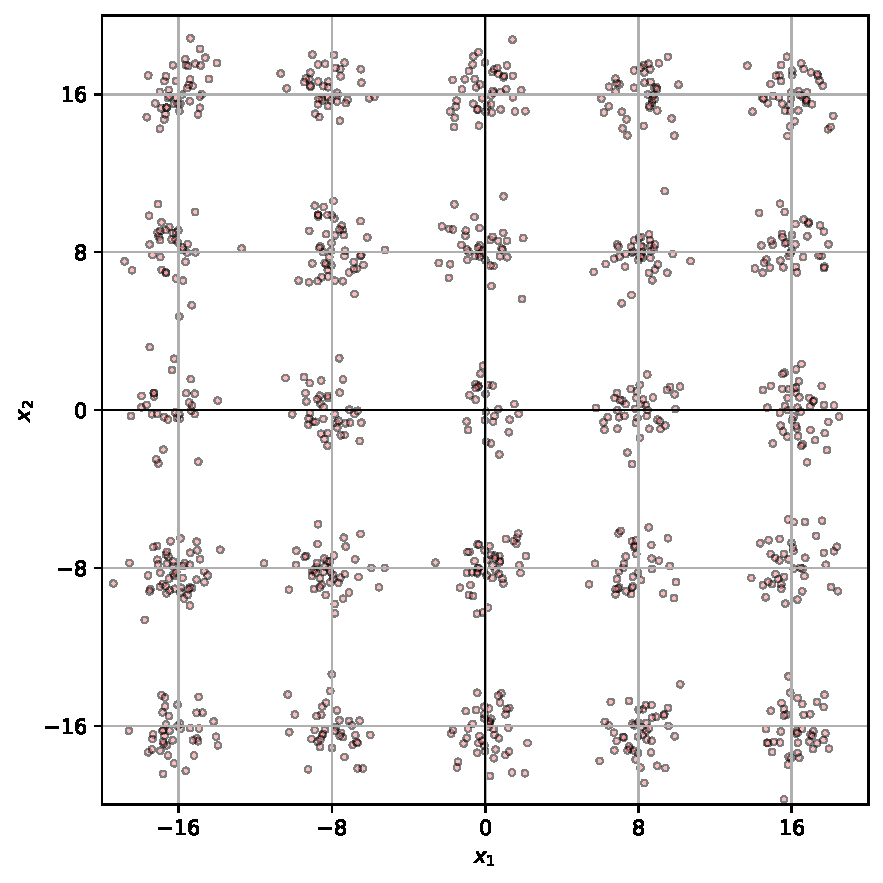
\includegraphics[width=\textwidth]{assets/gmm_prior_samples.pdf}
      \caption{GMM prior samples under DDPM with analytic score; $d_x = 8, d_y = 2$.}
      \label{fig:gmm-prior}
    \end{subfigure}
    \hfill
    \begin{subfigure}[b]{0.48\textwidth}
      \centering
      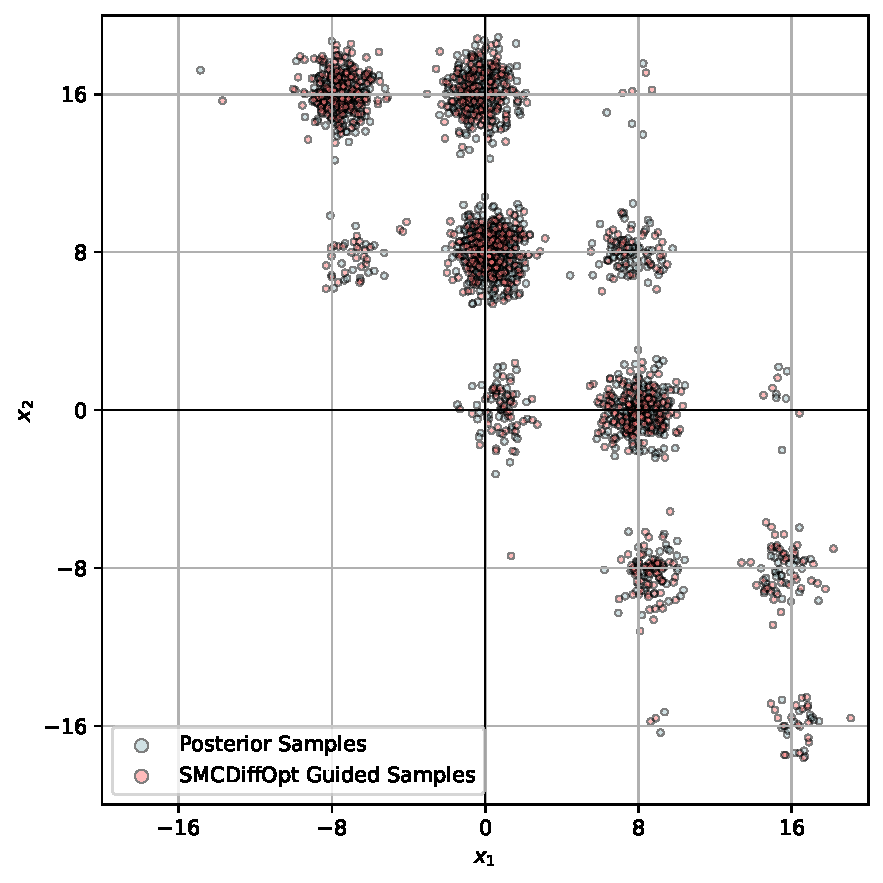
\includegraphics[width=\textwidth]{assets/gmm_smc_samples.pdf}
      \caption{\texttt{SMCDiffOpt} samples for a particular measurement model; $d_x = 8, d_y = 2$.}
      \label{fig:gmm-smc-samples}
    \end{subfigure}
    \caption{GMM Prior versus posterior samples under guidance through \texttt{SMCDiffOpt}.}
    \label{fig:gmm-prior-smc-samples}
\end{figure}

\begin{figure}[htbp]
    \centering
    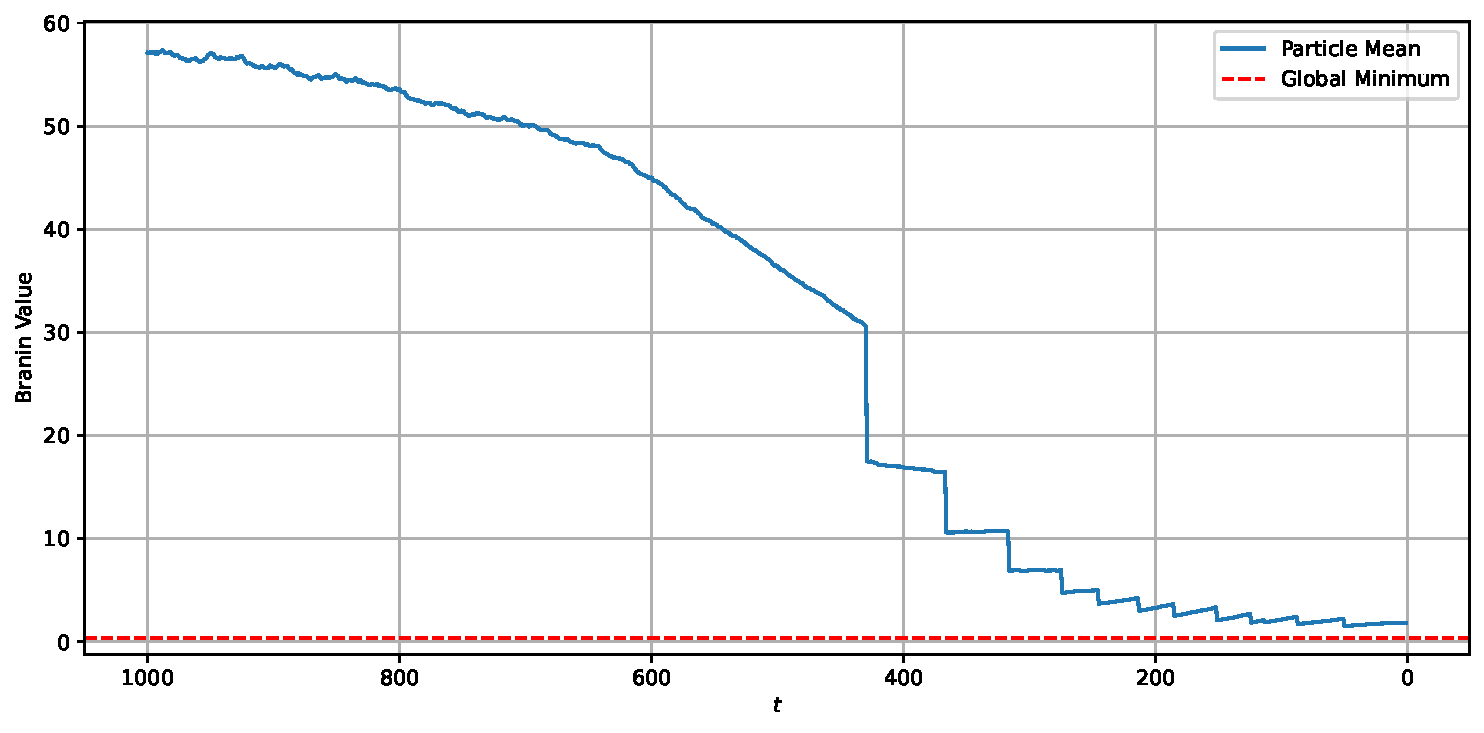
\includegraphics[width=1\textwidth]{assets/smc_branin_mean_val.pdf}
    \caption{Mean value of \autoref{eq:branin} on particles over time.}
    \label{fig:branin-mean-val}
\end{figure}

\begin{figure}[htbp]
    \centering
    \begin{subfigure}[b]{\textwidth}
      \centering
      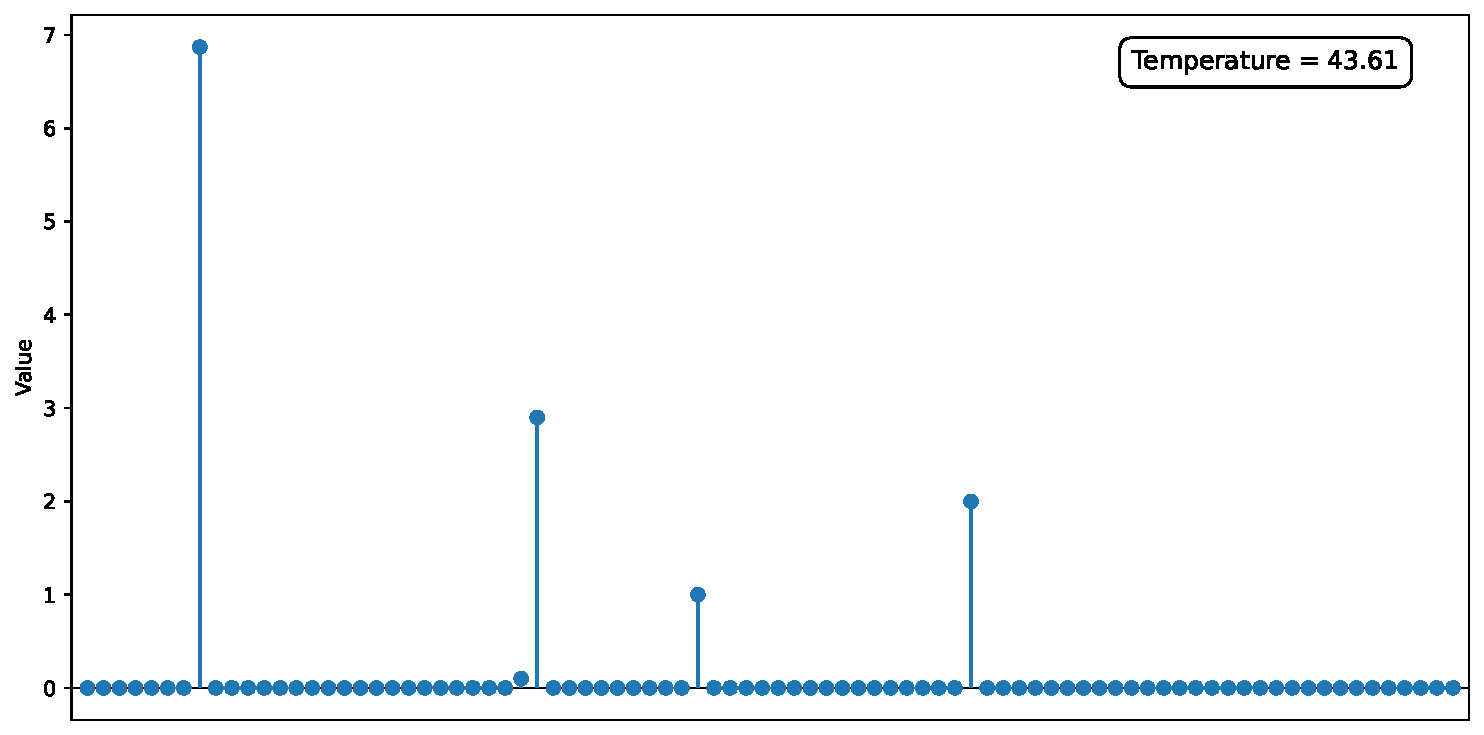
\includegraphics[width=0.8\textwidth]{assets/bb-real-sample.pdf}
      \caption{Real training sample.}
      \label{fig:bb-real}
    \end{subfigure}
    \begin{subfigure}[b]{\textwidth}
      \centering
      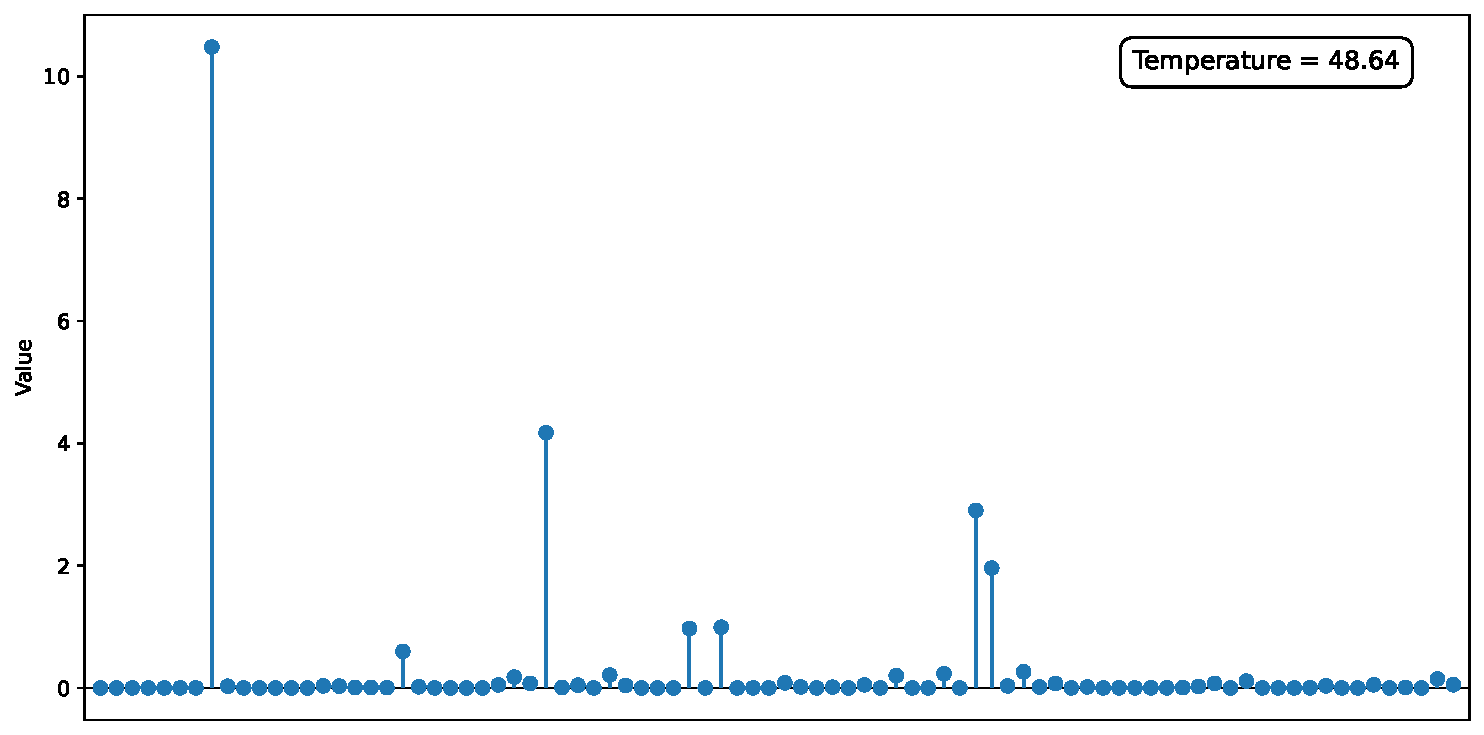
\includegraphics[width=0.8\textwidth]{assets/bb-unconditional-sample.pdf}
      \caption{Unconditionally generated sample from model.}
      \label{fig:bb-unconditional}
    \end{subfigure}
    \begin{subfigure}[b]{\textwidth}
        \centering
        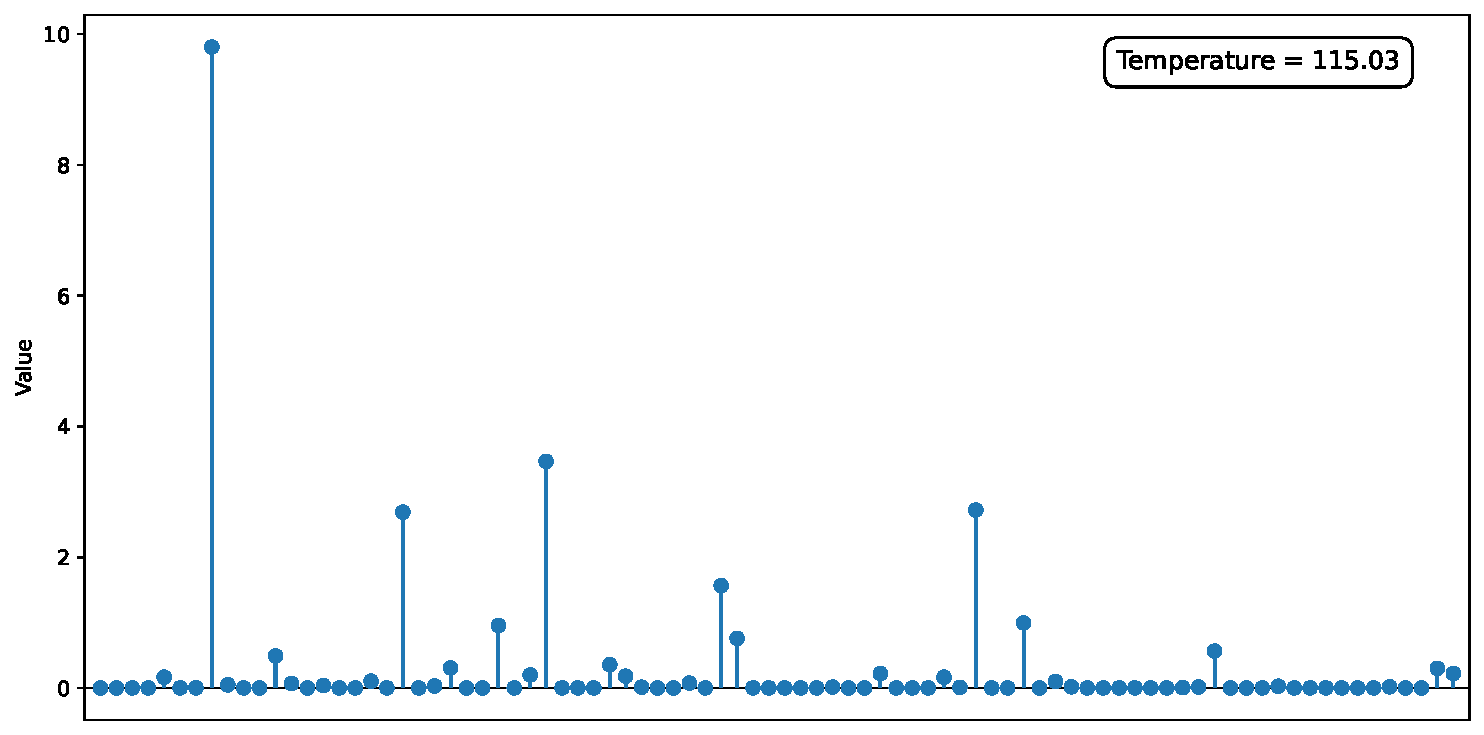
\includegraphics[width=0.8\textwidth]{assets/bb-optimised-sample.pdf}
        \caption{Optimised sample from running \texttt{SMCDiffOpt}.}
        \label{fig:bb-optimised}
      \end{subfigure}
    \caption{Real, synthetic, and optimised SuperConductor samples along with associated
    temperature values from evaluating configuration with oracle.}
    \label{fig:bb-samples}
\end{figure}

\newpage

\section{Proofs}\label{sec:proofs}

\begin{proof}[Proof of \autoref{prop:obs-gen}] \label{prf:obs-generation}
    Given
    \begin{align*}
        \mathbf{X}_t \mid \mathbf{X}_0 = \mathbf{x}_0 &\sim \mathcal{N}(c_t\cdot\mathbf{x}_0, d_t^2\cdot\mathbf{I}_{d_x}) \\
        \mathbf{Y}_t \mid \mathbf{Y}_0 = \mathbf{y}_0 &\sim \delta(\mathbf{y}_t - c_t\cdot \mathbf{y}_0) \\
        \mathbf{Y}_0 \mid \mathbf{X}_0 = \mathbf{x}_0 &\sim \mathcal{N}(A\mathbf{x}_t, \sigma_y^2\mathbf{I}_{d_y})
    \end{align*}
    we have
    \begin{align*}
        \EE{\mathbf{Y}_t \mid \mathbf{X}_0} &= \EE{\EE{\mathbf{Y}_t \mid \mathbf{Y}_0} \mid \mathbf{X}_0} \\
        &= \EE{c_t\cdot \mathbf{Y}_0 \mid \mathbf{X}_0} \\
        &= c_t\cdot A\mathbf{X}_0
    \end{align*}
    and
    \begin{align*}
        \VV{\mathbf{Y}_t \mid \mathbf{X}_0} &= \EE{\VV{\mathbf{Y}_t \mid \mathbf{Y}_0} \mid \mathbf{X}_0} + \VV{\EE{\mathbf{Y}_t \mid \mathbf{Y}_0} \mid \mathbf{X}_0} \\
        &= \VV{c_t\cdot \mathbf{Y}_0 \mid \mathbf{X}_0} \\
        &= c_t^2\sigma_y^2\cdot \mathbf{I}_{d_y}.
    \end{align*}
    Hence,
    \begin{equation*}
        \mathbf{Y}_t \mid \mathbf{X}_0 = \mathbf{x}_0 \sim \mathcal{N}(c_t\cdot A\mathbf{x}_0, \sigma_y^2c_t^2\cdot \mathbf{I}_{d_y}).
    \end{equation*}
    Further,
    \begin{align*}
        A\mathbf{X}_t \mid \mathbf{X}_0 = \mathbf{x}_0 &\sim \mathcal{N}(c_t\cdot A\mathbf{x}_0, d_t^2\cdot AA^\top) \\
        \implies \mathbf{Y}_t - A\mathbf{X}_t \mid \mathbf{X}_0 = \mathbf{x}_0 &\sim \mathcal{N}(0, \sigma_y^2c_t^2\cdot \mathbf{I}_{d_y} + d_t^2\cdot AA^\top) \\
        \implies \mathbf{Y}_t \mid \mathbf{X}_t = \mathbf{x}_t &\sim \mathcal{N}(A\mathbf{x}_t, \sigma_y^2c_t^2\cdot \mathbf{I}_{d_y} + d_t^2\cdot AA^\top)
    \end{align*}

\end{proof}

\begin{proposition}[Gaussian-Gaussian Exactness for Linear Observations] \label{prop:gaussian-exact}
    Suppose
    \begin{align*}
        \mathbf{X}_{t} \mid \mathbf{X}_{t+1} &\sim \mathcal{N}\left( \mathbf{\mu}_{t+1}(\mathbf{x}_{t+1}), \Sigma_{t+1} \right)  \\
        \mathbf{Y}_{t} \mid \mathbf{X}_{t} = \mathbf{x}_{t} &\sim \mathcal{N}\left( A\mathbf{x}_{t}, \Xi_{t} \right)
    \end{align*}
    Consider some proposal
    \begin{align*}
        p_{t}(\mathbf{x}_{t} \mid \mathbf{y}_{t}, \mathbf{x}_{t+1}) \propto p_{t}(\mathbf{x}_{t} \mid \mathbf{x}_{t+1})g_{t}(\mathbf{y}_{t} \mid \mathbf{x}_{t}).
    \end{align*}
    Then,
    \begin{align*}
        \mathbf{Y}_{t} \mid \mathbf{X}_{t+1} = \mathbf{x}_{t+1} \sim \mathcal{N}\left( A\mu_{t+1}, \Xi_{t} + A\Sigma_{t+1}A^\top \right).
    \end{align*}
\end{proposition}
\begin{proof}
    By Gaussian conjugacy, it immediately follows that
    \begin{align*}
        \mathbf{X}_{t} \mid \mathbf{Y}_{t} = \mathbf{y}_{t}, \mathbf{X}_{t+1} = \mathbf{x}_{t+1} &\sim \mathcal{N}\left( \mu_{t+1}^P, \Sigma_{t+1}^P \right) 
    \end{align*}
    where
    \begin{align*}
        \mu_{t+1}^P &= \Sigma_{t+1}^P\left( \Sigma_{t+1}^{-1}\mu_{t+1}(\mathbf{x}_{t+1}) + A^\top\Xi_{t}^{-1}\mathbf{y}_{t} \right) \\
        \Sigma_{t+1}^P &= \left( \Sigma_{t+1}^{-1} + A^\top \Xi_{t}^{-1}A \right)^{-1}.
    \end{align*}
    The normalizing constant of the proposal is
    \begin{align*}
        \int p_{t}(\mathbf{x}_{t} \mid \mathbf{x}_{t+1})g_{t}(\mathbf{y}_{t} \mid \mathbf{x}_{t}) \, d\mathbf{x}_{t} &= g_{t}(\mathbf{y}_{t} \mid \mathbf{x}_{t+1})
    \end{align*}
    Note that
    \begin{align*}
        \mathbb{E}\left\{ \mathbf{Y}_{t} \mid \mathbf{X}_{t+1} \right\} &= \mathbb{E}\left\{\mathbb{E}\left\{\mathbf{Y}_{t} \mid \mathbf{X}_{t}\right\} \mid \mathbf{X}_{t+1}\right\} &\dots\text{tower property} \\
        &= \mathbb{E}\left\{A\mathbf{X}_{t} \mid \mathbf{X}_{t+1}\right\} \\
        &= A\mathbb{E}\left\{\mathbf{X}_{t} \mid \mathbf{X}_{t+1}\right\} \\
        &= A\mu_{t+1}(\mathbf{X}_{t+1}) \\
        \mathbb{V}\left\{\mathbf{Y}_{t} \mid \mathbf{X}_{t+1}\right\} &= \mathbb{E}\left\{\mathbb{V}\left\{\mathbf{Y}_{t} \mid \mathbf{X}_{t}\right\} \mid \mathbf{X}_{t+1}\right\} + \mathbb{V}\left\{\mathbb{E}\left\{\mathbf{Y}_{t} \mid \mathbf{X}_{t}\right\} \mid \mathbf{X}_{t+1}\right\} &\dots \text{total variance} \\
        &= \mathbb{E}\left\{\Xi_{t} \mid \mathbf{X}_{t+1}\right\} + \mathbb{V}\left\{A\mathbf{X}_{t} \mid \mathbf{X}_{t+1}\right\} \\
        &= \Xi_{t} + A\mathbb{V}\left\{\mathbf{X}_{t} \mid \mathbf{X}_{t+1}\right\}A^{\top} \\
        &= \Xi_{t} + A\Sigma_{t+1}A^{\top}
    \end{align*}
    Since $\mathbf{Y}_{t}$ is an affine transformation, it follows then that:
    \begin{align*}
        \mathbf{Y}_{t} \mid \mathbf{X}_{t+1} = \mathbf{x}_{t+1} \sim \mathcal{N}\left( A\mu_{t+1}, \Xi_{t} + A\Sigma_{t+1}A^\top \right).
    \end{align*}
\end{proof}

\newpage

\section{Further Experimental Details} \label{sec:experimental-extra}

\paragraph{Gaussian Mixture Model} We aimed to include MCGdiff
\parencite{cardosoMonteCarloGuided2023} in our comparison. However, we were unable to reproduce
their results, even using the code on their repository. Indeed, we found that the resulting sliced
Wasserstein distances from MCGdiff were almost uniformly larger than those of
\text{SMCDiffOpt} on each experimental run (with identical setups and pseudo-RNG seeds). This
is doubly unexpected since the raw results don't align with those found in their paper,
and since theoretically their proposal should be more optimal than ours for this particular task;
if we take the values they give in Table 1 of their paper and compare them with those in
\autoref{tab:gmm} we see this is indeed the case. Given the time constraints, the exhaustion of all
obvious potential author-errors, and assuming the validity of their results, we opted to omit our
results from a comparison. However, we provide in \autoref{tab:gmm-mcg} the results including
MCGdiff but note with caution that we lack confidence in such figures.

\begin{table}[ht]
    \centering
    \begin{tabular}{llllllll}
        \toprule
        $\sigma_y$ & $d_x$ & $d_y$ & SMCDiffOpt & MCGDiff & DPS & $\Pi$IGD & TMPD \\
        \midrule
        \multirow[t]{6}{*}{0.0} & \multirow[t]{3}{*}{8} & 1 & 0.98 ± 0.44 & 0.95 ± 0.44 & 8.22 ± 7.32 & 3.15 ± 2.58 & 3.5 ± 2.67 \\
         &  & 2 & 0.55 ± 0.43 & 0.39 ± 0.33 & 0.41 ± 0.29 & 0.33 ± 0.27 & 0.44 ± 0.34 \\
         &  & 4 & 0.21 ± 0.07 & 0.15 ± 0.09 & 0.12 ± 0.06 & 0.09 ± 0.03 & 0.08 ± 0.04 \\
        \cline{2-8}
         & \multirow[t]{3}{*}{80} & 1 & 0.75 ± 0.31 & 1.06 ± 0.77 & 2.45 ± 1.79 & 3.18 ± 2.6 & 2.66 ± 1.47 \\
         &  & 2 & 1.22 ± 1.04 & 2.31 ± 2.21 & 1.35 ± 1.21 & 0.33 ± 0.27 & 0.81 ± 0.68 \\
         &  & 4 & 0.26 ± 0.05 & 2.22 ± 1.92 & 0.97 ± 0.86 & 0.08 ± 0.02 & 0.68 ± 0.44 \\
        \cline{1-8} \cline{2-8}
        \multirow[t]{6}{*}{0.1} & \multirow[t]{3}{*}{8} & 1 & 1.13 ± 0.51 & 0.79 ± 0.62 & 8.18 ± 7.5 & 3.22 ± 2.67 & 3.11 ± 2.31 \\
         &  & 2 & 0.2 ± 0.07 & 1.15 ± 1.09 & 0.38 ± 0.28 & 0.19 ± 0.13 & 0.43 ± 0.34 \\
         &  & 4 & 0.15 ± 0.05 & 0.25 ± 0.12 & 0.16 ± 0.06 & 0.07 ± 0.01 & 0.06 ± 0.01 \\
        \cline{2-8}
         & \multirow[t]{3}{*}{80} & 1 & 1.25 ± 1.02 & 1.26 ± 0.87 & 2.51 ± 2.11 & 2.93 ± 2.56 & 2.56 ± 1.18 \\
         &  & 2 & 0.45 ± 0.32 & 3.06 ± 2.93 & 1.27 ± 1.14 & 0.62 ± 0.56 & 0.66 ± 0.54 \\
         &  & 4 & 0.23 ± 0.06 & 3.34 ± 3.01 & 1.03 ± 0.9 & 0.08 ± 0.02 & 0.63 ± 0.34 \\
        \cline{1-8} \cline{2-8}
        \multirow[t]{6}{*}{1.0} & \multirow[t]{3}{*}{8} & 1 & 1.35 ± 1.0 & 1.14 ± 0.7 & 6.62 ± 4.96 & 1.16 ± 0.72 & 1.35 ± 0.9 \\
         &  & 2 & 0.44 ± 0.28 & 1.11 ± 1.04 & 2.92 ± 2.42 & 0.94 ± 0.89 & 1.44 ± 1.15 \\
         &  & 4 & 0.15 ± 0.03 & 0.12 ± 0.06 & 1.19 ± 0.66 & 0.1 ± 0.03 & 0.45 ± 0.26 \\
        \cline{2-8}
         & \multirow[t]{3}{*}{80} & 1 & 1.69 ± 1.37 & 1.49 ± 0.75 & 5.26 ± 4.4 & 1.2 ± 0.79 & 1.23 ± 0.53 \\
         &  & 2 & 0.89 ± 0.78 & 2.08 ± 1.97 & 3.21 ± 2.95 & 1.68 ± 1.62 & 1.41 ± 1.16 \\
         &  & 4 & 1.12 ± 0.92 & 4.52 ± 2.55 & 1.54 ± 0.99 & 0.89 ± 0.74 & 1.37 ± 0.67 \\
        \cline{1-8} \cline{2-8}
        \bottomrule
    \end{tabular}
    \caption{Sliced-Wasserstein distances for GMM experiment with MCGdiff included. These results
    do not align with those in \textcite{cardosoMonteCarloGuided2023}, despite running exactly
    the script in their repository.}
    \label{tab:gmm-mcg}
\end{table}

\paragraph{Branin Optimisation} We train a noise estimating neural network and then employ
REF to convert it to a score approximating network, $s_\theta(\mathbf{x}_t, t)$.
The model is a 4 layer MLP with 256 hidden dimensions in each layer and ReLU activation function.
We also add some simple Fourier based time embeddings to encode the current time-step. The model
is trained on 6000 datapoints --- uniformly sampled from the elliptical region of interest --- in
20,000 epochs. We use an Adam optimiser for training model parameters with a base learning rate of
$10^{-3}$. The diffusion is parametrised with $\beta_{\text{min}}=10^{-4}$,
$\beta_{\text{max}}=0.02$, $T=1000$, with linear schedule and applying DDPM sampling.

\paragraph{SuperConductor Optimisation} Our model architecture is essentially identical to that used
in the Branin optimisation. For training, we used a 90:10 train:evaluation split of the 17,014
subset of vectors, using a 256 batch size in 40,000 epochs, monitoring evaluation loss for early
stopping. We use an AdaBelief optimiser for training model parameters with a base learning rate of
$3\times 10{-4}$. We similarly parametrise the diffusion as in the Branin experiment.

\newpage

\section{Additional Background and Related Works} \label{sec:extra}

\subsection{Diffusion Models}

\begin{remark}[SDE Representation] \label{rem:sde-rep}
    The DDPM approach corresponds to a discretised time rescaled Ornstein-Uhlenbeck process
    \parencite{boysTweedieMomentProjected2023,songScoreBasedGenerativeModeling2021}:
    $$
    d\mathbf{x}_t = -\frac{1}{2}\beta(t)\mathbf{x}_t dt + \sqrt{\beta(t)}d\mathbf{w}_t
    $$
    and is often referred to as the variance-preserving SDE
    \parencite{songScoreBasedGenerativeModeling2021}. When it comes to sampling, we can then
    analytically reverse the diffusion model using the result of
    \textcite{andersonReversetimeDiffusionEquation1982} and use any numeric sampler. The choice
    of sampling strategy corresponds to slightly different discretised equivalents and is discussed
    in detail in \textcite{songScoreBasedGenerativeModeling2021} in detail.
    Regardless, this SDE representation is what analytically justifies the backwards process
    (see \autoref{ftnt:sde-rep}).
\end{remark}

\begin{remark}[DDIM Representation] \label{rem:ddim}
    Under DDIM, take
    \begin{equation*}
        u_t = \sqrt{\alpha_{t-1}} \quad
        v_t = -\sqrt{1 - \overline{\alpha}_{t-1} - \sigma_t^2}\sqrt{1 - \overline{\alpha}_t} \quad
        w_t = \sigma_t
    \end{equation*}
    with $\{\sigma_t\}_{t=1}^T$ an arbitrary conditional variance sequence. It's common to consider
    \begin{equation*}
        \sigma_t(\eta) = \eta\sqrt{\frac{1 - \alpha_{t-1}}{1 - \alpha_t}}\sqrt{1 - \frac{\alpha_t}{\alpha_{t-1}}},\quad \eta \in [0,1]
    \end{equation*}
    with $\eta=1$ ultimately reducing $u_t, v_t, w_t$ to the DDPM values, and $\eta=0$ corresponding
    to deterministic generation \parencite{songDenoisingDiffusionImplicit2020}.
\end{remark}

\begin{remark}[Time Respacing] \label{rem:time-respacing}
    One of the remarkable features of the DDIM algorithm is it enabling \emph{time re-spacing}
    whereby we can sample from the backwards process in fewer time-steps. In this paper, we don't
    consider such re-spacing though in principle our methodology does not prohibit it.
\end{remark}

\begin{proposition}[Score to Noise Conversion] \label{prop:score-to-noise}
    Let $\mathbf{x}_t = c_t\mathbf{x}_0 + d_t\epsilon_t$ be a forward noised observation. Then
    $$
    \nabla_{\mathbf{x}_t} \log q_t(\mathbf{x}_t) \approx -\frac{\mathbf{\epsilon}_t}{d_t}.
    $$
\end{proposition}
\begin{proof}
    Follows from forward marginal and Tweedie's formula (\autoref{eq:tweedie}).
\end{proof}

\subsection{Non-Linear Case} \label{sec:non-linear}

In the case of non-linear measurement operator, $m$, we must resort to approximate methods.
Assuming $\mathbf{X}_0 \mid \mathbf{X}_t$ is Gaussian (this is the \emph{Moment Projection}
assumption \parencite{boysTweedieMomentProjected2023}), we can easily show:
\begin{equation*}
    \mathbf{Y}_t \mid \mathbf{X}_t = \mathbf{x}_t \sim \mathcal{N}\left(c_t\cdot\EE{m(\mathbf{X}_0) \mid \mathbf{X}_t = \mathbf{x}_t}, c_t^2\left(\sigma_y^2\cdot \mathbf{I}_{d_y} + \VV{m(\mathbf{X}_0) \mid \mathbf{X}_t = \mathbf{x}_t}\right)\right)
\end{equation*}
and then use a first-order Taylor expansion (linearisation) so that
\begin{eqnarray}
    m(\mathbf{X}_0) \approx m(\mu_{\mathbf{X}_0 \mid \mathbf{X}_t}) + \nabla m(\mu_{\mathbf{X}_0 \mid \mathbf{X}_t})\cdot (\mathbf{X}_0 - \mu_{\mathbf{X}_0 \mid \mathbf{X}_t})
\end{eqnarray}
to approximate the likelihood by:
\begin{equation*}
    \mathbf{Y}_t \mid \mathbf{X}_t = \mathbf{x}_t \sim \mathcal{N}\left(c_t\cdot m(\mu_{\mathbf{X}_0 \mid \mathbf{X}_t}), c_t^2\left(\sigma_y^2\cdot \mathbf{I}_{d_y} + \nabla m(\mu_{\mathbf{X}_0 \mid \mathbf{X}_t})\Sigma_{\mathbf{X}_0 \mid \mathbf{X}_t}\nabla m(\mu_{\mathbf{X}_0 \mid \mathbf{X}_t})^\top\right)\right)
\end{equation*}
where $\mu_{\mathbf{X}_0} \approx \hat{\mathbf{x}}_0(\mathbf{x}_t)$, and we approximate
$\Sigma_{\mathbf{X}_0 \mid \mathbf{X}_t}$ by $r_t^2\mathbf{I}_{d_x}$ with $r_t^2$ fixed based on
the diffusion parameters \parencite{hoDenoisingDiffusionProbabilistic2020} or learnt
\parencite{nicholImprovedDenoisingDiffusion2021}, or better approximated with a second-order
Tweedie formula \parencite{boysTweedieMomentProjected2023}.

Alternatively, we can make the approximate assumption $\mathbf{X}_t \approx c_t\mathbf{X}_0$, so
that
\begin{equation*}
    \mathbf{Y}_t \mid \mathbf{X}_t = \mathbf{x}_t \sim \mathcal{N}\left(c_t\cdot m\left(\frac{\mathbf{x}_t}{c_t}\right), c_t^2\sigma_y^2\mathbf{I}_{d_y}\right).
\end{equation*}
Referring to \ref{eq:obs-likelihood}, this essentially ignores the second term in the variance.
More concretely, it assumes we deterministically `noise' the data exactly as in \ref{eq:obs-gen}.
This approximation can work well in cases where $g$ is not significantly non-linear, such as in
\autoref{sec:gmm}.

\subsection{FPS-SMC Observation Noising}

Rather than \autoref{eq:obs-gen}, \textcite{douDiffusionPosteriorSampling2023} instead considers
a ``shared-noise'' or ``duplex'' diffusion.

\begin{proposition}[Obvservation Diffusion] \label{prop:obs-diffusion}
    \textcite[Proposition B.1]{douDiffusionPosteriorSampling2023}.
    Let $\mathbf{x}_t$ be generated according to the forward marginal of some diffusion process.
    Let $\mathbf{y} = \mathbf{y}_0$ be some (linear) measurement we have about the clean sample,
    $\mathbf{x}_0$. Construct a sequence $\{\mathbf{y}_t\}_{t=1}^T$ by
    \begin{equation*}
        \mathbf{y}_t = a_t\cdot \mathbf{y}_{t-1} + b_t\cdot A\epsilon_t,\quad \epsilon_t \sim \mathcal{N}(0, \mathbf{I}_{d_y})
    \end{equation*}
    where $\epsilon_t$ is the \emph{same} as used for forward noising $\mathbf{x}_0$ at time-step $t$.
    It follows that
    \begin{equation}
        \mathbf{Y}_t \mid \mathbf{X}_t = \mathbf{x}_t \sim \mathcal{N}(A\mathbf{x}_t, \sigma_y^2c_t^2\cdot \mathbf{I}_{d_y}) \label{eq:obs-likelihood-dou}
    \end{equation}
    with $g(\mathbf{y}_0 \mid \mathbf{x}_0) = g(\mathbf{y} \mid \mathbf{x}_0) = \mathcal{N}(\mathbf{y}; A\mathbf{x}_0, \sigma_y^2\cdot \mathbf{I}_{d_y})$
    exactly the measurement density.
\end{proposition}

Note because of the noise-sharing, we get cancellation in the covariance of the likelihood, dropping
the $d_t^2\cdot AA^\top$ term as in \autoref{eq:obs-likelihood}.

Based on \autoref{prop:obs-diffusion} and \textcite[Remark B.1]{douDiffusionPosteriorSampling2023},
we can generate some $\{\mathbf{y}_t\}_{t=0}^T$ either forwards or \emph{backwards}.
The latter follows because where in the backwards process for $\mathbf{x}_t$ we use an estimate of
$\mathbf{x}_0$ (via Tweedie's formula), for the observations we have $\mathbf{y}_0$, and an
expression can be analytically derived.
